In this chapter I will give an overview of how this audio codec will be designed, and explaining the various decisions I made along the way.

I have decided to call this new codec \emph{ANMF} (stands for Audio-NMF), using files with the extension \emph{.anmfx}, where \emph{x} represents the compression method. It will be implemented as a command line utility.

There are currently three different ANMF formats that you can choose from, and their main difference is which audio representation is being compressed by NMF. They are as follows:

\begin{description}
	\item[ANMF-RAW] denoted by \emph{r}, compresses the signal in PCM form (time domain)
	\item[ANMF-MDCT] denoted by \emph{m}, compresses the signal transformed with MDCT (frequency domain)
	\item[ANMF-STFT] denoted by \emph{s}, compresses the signal transformed with STFT (frequency domain)
\end{description}

\section{WAVE file}
WAVE, WAV or Waveform audio is a file format for storing digitized audio, created as a joint design by the Microsoft Corporation and the IBM Corporation. They are built on top of the chunk-based RIFF format. For details on the specific structure of a WAVE file please refer to \cite{sapp_pcm}.

It stores raw uncompressed audio samples in PCM format along with some metadata and will serve as both the standard input and output to the ANMF codec. Most commonly used formats can be converted to and from WAV as well and thus it will serve as a good baseline.

Samples in this format can be represented by different datatypes, I chose 16-bit signed integers, i.e. each sample's amplitude is represented by a whole number between $-32768$ and $32767$. The sample rate can vary, but a good standard value the experiments will use is $44.1$ kHz, which corresponds to audio CD quality.

\section {ANMF File structure}
The base container for the compressed ANMF file is the same no matter which encoding method you use. The bytes are saved in little endian byte order.

Please refer to Table \ref{tab:anmf_file} and each encoding method's table for the specific file structure. The first eleven bytes are mostly set in stone other than the method specification, but after that it varies greatly.

\begin{table}[htbp]\caption{ANMF file structure}
	\label{tab:anmf_file}
	\centering
	\begin{tabular}{|c|c|l|}
		\hline
		Bytes & Data type & Description \\ \hline
		0-3 & char[] & identifier string "ANMF" \\
		4 & char & method used, can be 'S', 'R' or 'M' \\
		5-6 & uint16 & \# of channels \\
		7-10 & uint32 & sample rate \\
		11-? & enc\_data & encoded data depending on the method \\
		\hline
	\end{tabular}
\end{table}

When serializing matrices to a file, the structure in Table \ref{tab:anmf_serial_matrix} will be used, denoted by a "matrix($dt$)" datatype in the following tables, where $dt$ stands for the datatype used for the matrix elements.

\begin{table}[htbp]\caption{Serialized matrix structure}
	\label{tab:anmf_serial_matrix}
	\centering
	\begin{tabular}{|c|c|l|}
		\hline
		Bytes (relative) & Data type & Description \\ \hline
		0-3 & uint32 & amount of rows in the matrix \\
		4-7 & uint32 & amount of columns in the matrix \\
		8-($8+x-1$) & $dt$ & row-wise values of the matrix, $x = rows*columns$ \\
		\hline
	\end{tabular}
\end{table}

There's also one more kind of matrix, a matrix using Huffman encoded quantized values. This will be denoted by a "quant\_matrix" datatype. For its specification please see Table \ref{tab:anmf_serial_quant_matrix}.

\begin{table}[htbp]\caption{Serialized quantized matrix structure}
	\label{tab:anmf_serial_quant_matrix}
	\centering
	\begin{tabular}{|c|c|l|}
		\hline
		Bytes (relative) & Data type & Description \\ \hline
		0-3 & uint32 & amount of rows in the matrix \\
		4-7 & uint32 & length $L$ of the Huffman encoded byte stream \\
		8-($8+L-1$) & byte[] & Huffman encoded byte stream representing the matrix \\
		\hline
	\end{tabular}
\end{table}

\section{Encoder}
The encoder is responsible for taking a raw audio file and encoding the data within, producing a compressed version of the original. Please refer to Figure \ref{fig:design_encoder} for a visual representation of the process.

\begin{figure}[ht]
	\caption[Encoder overview]{A high level overview of the ANMF audio encoder.}
	\label{fig:design_encoder}
	\centering
	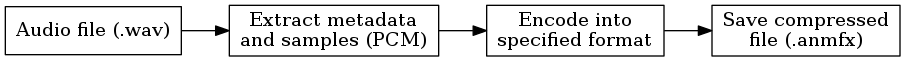
\includegraphics[width=\textwidth]{design_encoder.png}
\end{figure}

Next, each format's encoding process will be outlined (third step in the figure). If the audio file has multiple channels, this process is repeated on each channel separately.

\subsection{ANMF-RAW}
\begin{figure}[ht]
	\caption[ANMF-RAW Encoder]{The encoding scheme for ANMF-RAW.}
	\label{fig:encoding_nmf_raw}
	\centering
	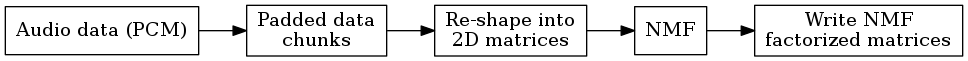
\includegraphics[width=\textwidth]{nmf_raw.png}
\end{figure}

ANMF-RAW works on the principle of applying NMF directly to the PCM audio samples $x_n$. However, the samples are initially an array of 16-bit signed integers, and as such, they need to be processed first before NMF can be used.

A chunk shape is specified to determine how many rows and columns each matrix will have before NMF. We choose a target matrix shape of $1152 \times 200$ to match the amount of samples per frame in the other methods.The sample array is then padded with zeroes to ensure there are enough elements at the end of the array to ensure every matrix can have the same shape and number of elements. The amount of padding must be written to the output so that we know the length of the original array when decoding.

Once the array is padded, we iterate over the samples and split them into equal chunks of size $rows*columns$. This array is then "folded" to produce a matrix of the desired shape. We then obtain a matrix of signed integers, so in order to be able to use NMF, we first need to get rid of all the negative values. To do that, we increment each chunk by the absolute value of its smallest element, guaranteeing that the lowest value in the matrix is $\ge 0$.

Once we have this matrix, we proceed by applying basic random-initialized Euclidean-based NMF on it, obtaining the basis matrix $W$ and coefficient matrix $H$. Lastly, for each chunk, we write the value we incremented the matrix by, and the two decomposition matrices.

\begin{table}[htbp]\caption{ANMF-RAW data structure}
	\label{tab:anmf_raw_file}
	\centering
	\begin{tabular}{|c|c|l|}
		\hline
		Bytes (relative) & Data type & Description \\ \hline
		0-3 & uint32 & amount of zeroes used to pad the samples \\
		4-7 & uint32 & amount of chunks \\
		8-? & data\_chunk[] & NMF-compressed data chunks (refer to Table \ref{tab:anmf_raw_data}) \\
		\hline
	\end{tabular}
\end{table}

\begin{table}[htbp]\caption{ANMF-RAW structure of each data chunk}
	\label{tab:anmf_raw_data}
	\centering
	\begin{tabular}{|c|c|l|}
		\hline
		Bytes (relative) & Data type & Description \\ \hline
		0-7 & float64 & absolute value that the matrix was incremented by \\
		8-? & matrix(float32) & matrix $W$ \\
		?-? & matrix(float32) & matrix $H$ \\
		\hline
	\end{tabular}
\end{table}

\subsection{ANMF-MDCT}
\begin{figure}[ht]
	\caption[ANMF-MDCT Encoder]{The encoding scheme for ANMF-MDCT.}
	\label{fig:encoding_nmf_mdct}
	\centering
	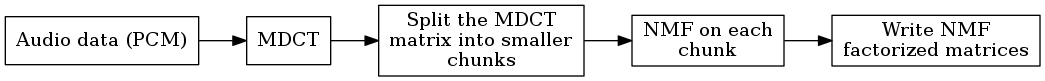
\includegraphics[width=\textwidth]{nmf_mdct.png}
\end{figure}

In ANMF-MDCT, as the name suggests, the PCM input will be transformed using MDCT as per Section \ref{sec:mdct}. Since this is a lapped transform, each transformed block will have a 50\% overlap with the following block. We choose a frame size of $2N = 1152$ and split the signal into blocks of that size, thus each block will contain $N = 576$ coefficients from its own block, and another $576$ from the following one.

The decision to have a block size of $N = 576$ stems from the fact that this will give us the same amount of frequency resolution that e.g. MP3 uses (as seen in Section \ref{sec:mp3}), which proved to be enough for human hearing.

As before, we first pad the signal at the end with zeroes to align it to the desired block size. To prevent loss of data in the first and the last block due to the overlapping, we further pad the signal by an array of zeroes, equal in size to the size of a block, that is $N$ zeroes both at the beginning and the end of the signal.

Then, we apply a windowing function on each block to bring the values near the edges closer to $0$ to help mitigate spectral leakage. We use the MLT window $w_n^M$ as defined in Section \ref{sec:mlt}.

Finally, we apply the MDCT on each of the windowed blocks and obtain a matrix of MDCT coefficients in the form of real numbers.

This matrix is then split into smaller chunks. For example, if the MDCT matrix contains $576$ rows and $1100$ columns, we might split it into submatrices sized $576 \times 200$, with the last one being $576 \times 100$, as no padding is necessary here. This amount of chunks is written to the output. Basic random-initialized Euclidean-based NMF is then ran on each of the chunks separately and the decomposition matrices serialized.

\begin{table}[htbp]\caption{ANMF-MDCT data structure}
	\label{tab:anmf_mdct_file}
	\centering
	\begin{tabular}{|c|c|l|}
		\hline
		Bytes (relative) & Data type & Description \\ \hline
		0-3 & uint32 & amount of zeroes used to pad the samples \\
		4-7 & uint32 & amount of MDCT submatrix chunks \\
		8-? & data\_chunk[] & NMF-compressed MDCT chunks (refer to Table \ref{tab:anmf_mdct_data}) \\
		\hline
	\end{tabular}
\end{table}

\begin{table}[htbp]\caption{ANMF-MDCT structure of each data chunk}
	\label{tab:anmf_mdct_data}
	\centering
	\begin{tabular}{|c|c|l|}
		\hline
		Bytes (relative) & Data type & Description \\ \hline
		0-7 & float64 & absolute value that the matrix was incremented by \\
		8-? & matrix(float32) & matrix $W$ \\
		?-? & matrix(float32) & matrix $H$ \\
		\hline
	\end{tabular}
\end{table}

\subsection{ANMF-STFT}
\begin{figure}[ht]
	\caption[ANMF-STFT Encoder]{The encoding scheme for ANMF-STFT.}		\label{fig:encoding_nmf_stft}
	\centering
	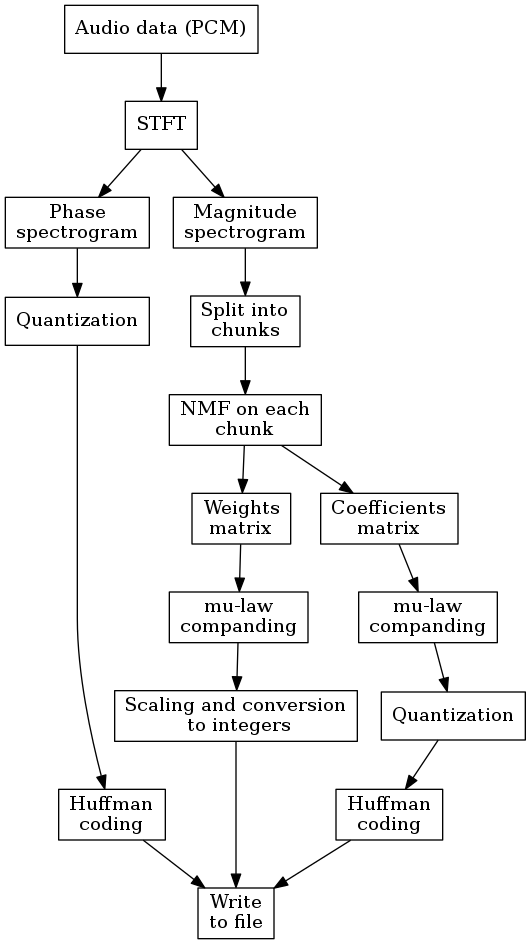
\includegraphics[width=0.6\textwidth]{nmf_stft.png}
\end{figure}

The design of ANMF-STFT is based on the solution suggested in \cite{nikunen_2010} with some changes along with only utilizing open source solutions.

Like with ANMF-MDCT, we choose a frame size of $N = 1152$, leading to a frequency resolution of $576$ bins. We begin by properly padding the signal to $N$ so that it's possible to be split into equal parts. We then use STFT with 50\% overlap and a block size of $N$, which means we end up with twice the coefficients compared to MDCT, but this is not a major issue.

During STFT, we must again window each block, leading to overlapping windows. We use the Hann window $w_n^H$ for this (as defined in Section \ref{sec:hann}).

Once STFT is finished, we end up with a matrix of Fourier transform coefficients in the form of complex numbers. Trying to apply NMF on the complex numbers directly would yield similar results to ANMF-MDCT, so we have to approach this differently.

If we visualise the complex valued elements in the complex plane, we can instead represent each element $z$ as two separate values:

\begin{description}
	\item[magnitude] also called the modulus, geometrically it's the distance from 0
	\item[phase] also called the argument, geometrically it's the angle from the real axis
\end{description}

To obtain the phase $\phi$ of a complex number $z = x + iy$, we can use the following formula:

\begin{align}
\phi(z) = \arg(z) = \arctantwo(y,x)
\end{align}

And to obtain the magnitude $|z|$ of the complex number:

\begin{align}
|z| = \sqrt{x^2 + y^2}
\end{align}

By calculating the magnitude and phase of every element in the STFT matrix individually, we obtain the magnitude spectrogram and the phase spectrogram respectively. We now need to encode both of them individually.

For the phase matrix, my experiments showed that applying NMF on it leads to a very noticeable loss in quality, so instead I opted for a different solution that ultimately ends up saving more space than NMF would.

The phase matrix contains values ranging from $-\pi$ to $\pi$. These values are uniformly quantized into 8 levels ($n_p = 3$ bits) as per Section \ref{sec:unif_quant}. Due to the relative frequency of the boundary values $-\pi$ and $\pi$, a mid-tread quantizer is used. The frequency of each quantization level is visible in Figure \ref{fig:stft_phase_quant_freq}.

Using these frequencies, we are able to then construct a Huffman coding table (refer to Section \ref{sec:huffman}) and use it to losslessly encode the quantized phase matrix using at most 4 bits per value.

\begin{figure}[ht]
	\caption[ANMF-STFT quantized phase frequencies]{Frequency of each quantization level in the phase spectrogram. Data taken from the average of all the example audio files.}
	\label{fig:stft_phase_quant_freq}
	\centering
	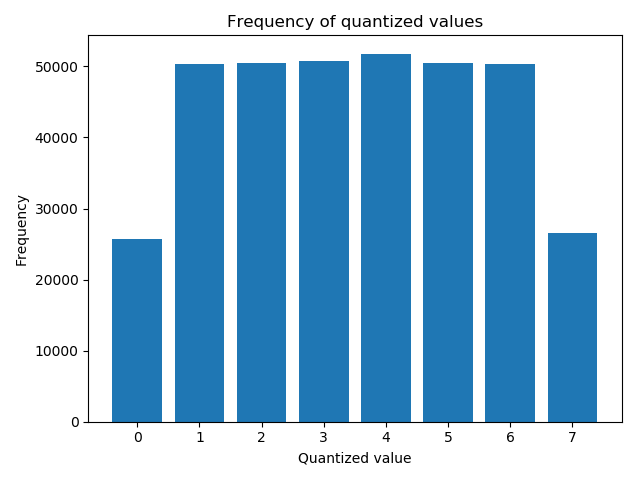
\includegraphics[width=\textwidth]{stft_phase_quant_freq.png}
\end{figure}

The magnitude spectrogram is where we actually use NMF. As it is effectively a matrix of signal amplitudes, it's less prone to noticeable quality loss if the values deviate a little. We split the magnitude matrix column-wise into smaller submatrices, e.g. $chunk_size = 500$.

On each submatrix we then run basic random-initialized Euclidean-based NMF, obtaining the weight matrix $W$ and coefficient matrix $H$.

For the next step, we apply $\mu$-law compression to both the decomposition matrices, as defined in Section \ref{sec:mulaw}. In order to be able to do that, we first scale both matrices to the range $[0, 1]$. We do this by applying the following formula to all elements in both matrices:

\begin{align}
M'_{ij} = \frac{M_{ij} - \min(M)}{|\max(M) - \min(M)|}
\end{align}

To restore the original scale later, we need to save both the minimum and maximum value, otherwise they will be lost in the non-uniform quantization.

For the $\mu$-law compression, we experiment with the value of $\mu$ later, but a good start is $\mu_W = 10^4$ and $\mu_H = 10^5$. We do this because we want to lower the amount of bits needed to represent each value, without losing the values near zero - that would lead to a large loss of quality, or in some cases, loss of the signal itself.

In the weight matrix, we then convert the compressed values into 32-bit unsigned integers, as going to values below that proved to cause loss of signal data, and this integer matrix is then serialized into the file.

However, in the case of the coefficient matrix $H$, we can go a lot further. We use a uniform quantizer with 32 levels ($n_h = 5$ bits) and we opt for a mid-tread quantizer again, as we want to be able to reconstruct a value of $0$, i.e. feature not present.

Similarly to the phase matrix, we take these quantized values and look at their frequencies. The results of this analysis are visible on Figure \ref{fig:stft_quant_freq}.

\begin{figure}[ht]
	\caption[ANMF-STFT quantized magnitude coefficient frequencies]{Frequency of each quantization level in the decomposed coefficients matrix of the magnitude spectrogram. Data taken from the average of all the example audio files.}
	\label{fig:stft_quant_freq}
	\centering
	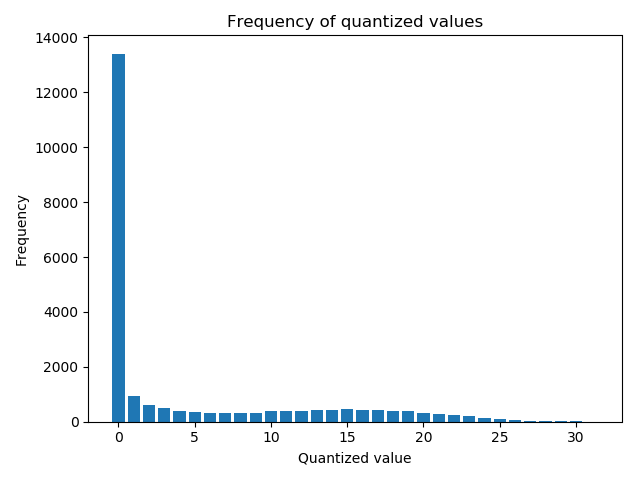
\includegraphics[width=\textwidth]{stft_quant_freq.png}
\end{figure}

Using this information, we can construct another Huffman coding table, separate for this matrix. As we can see, even despite the $\mu$-law compression, a lot of values still fall to a quantized value of $0$.

In a Huffman table from these frequencies, we then assemble the shortest code to the value $0$, i.e. we only need 1 bit. The longest code in a table constructed this way for 32 levels of quantization will only require 11 bits. Overall, we save a lot of space saving the matrix this way as opposed to storing the values as 32-bit floats or integers.

\begin{table}[htbp]\caption{ANMF-STFT data structure}
	\label{tab:anmf_stft_file}
	\centering
	\begin{tabular}{|c|c|l|}
		\hline
		Bytes (relative) & Data type & Description \\ \hline
		0-3 & uint32 & amount of zeroes used to pad the samples \\
		4-7 & uint32 & amount of STFT submatrix chunks \\
		8-? & quant\_matrix & quantized phase matrix \\
		?-? & data\_chunk[] & NMF-compressed magnitude chunks (refer to Table \ref{tab:anmf_stft_data}) \\
		\hline
	\end{tabular}
\end{table}

\begin{table}[htbp]\caption{ANMF-STFT structure of each magnitude submatrix}
	\label{tab:anmf_stft_data}
	\centering
	\begin{tabular}{|c|c|l|}
		\hline
		Bytes (relative) & Data type & Description \\ \hline
		0-7 & float64 & absolute value that the matrix was incremented by \\
		8-15 & float64 & minimum value before scaling to $[0, 1]$ \\
		16-23 & float64 & maximum value before scaling to $[0, 1]$ \\
		24-? & matrix(uint32) & $\mu$-law compressed matrix $W$ \\
		?-? & quant\_matrix & quantized $\mu$-law compressed matrix $H$ \\
		\hline
	\end{tabular}
\end{table}

\subsubsection{Huffman encoding}
\label{sec:huffman}
Huffman code refers to an optimal prefix coding scheme often employed for lossless compression. It's used to compress a message that only consists of members from a finite, known beforehand set of symbols. \cite{huffman_1952}

The goal is to create a dictionary that maps each value to a sequence of bits, where none of the sequences is a prefix of another one, which means that there are no ambiguities when decoding a Huffman encoded message, and we do not need to store any information about where one code begins and where it ends.

The main characteristic of a Huffman code is that the more frequent a symbol is, the shorter code it will be assigned. So in the case of a system where a certain symbol is very frequent, a message consisting of mostly those symbols will be compressed greatly, with no loss of data.

\begin{algorithm}[h]
\caption{Huffman code compression}
\label{alg:huffman}
\KwIn{a list of symbols and their probabilities}
\KwOut{a Huffman tree}
queue $\leftarrow$ new PriorityQueue()\;
\ForEach{item x in input}{
	node $\leftarrow$ new Node()\;
	node.symbol $\leftarrow$ x.symbol\;
	node.prob $\leftarrow$ x.probability\;
	node.leftChild, node.rightChild $\leftarrow$ null\;
	queue.enqueue(node, node.prob)\;
}
\While{queue.length $>$ 1}{
	node1 $\leftarrow$ queue.dequeue()\;
	node2 $\leftarrow$ queue.dequeue()\;
	newNode $\leftarrow$ new Node()\;
	newNode.leftChild $\leftarrow$ node1\;
	newNode.rightChild $\leftarrow$ node2\;
	newNode.prob $\leftarrow$ node1.prob + node2.prob\;
	queue.enqueue(newNode, newNode.prob)\;
}
\end{algorithm}

Algorithm \ref{alg:huffman} describes the compression process, at the end of which we obtain a Huffman tree. By traversing this tree from the root and assigning every left child a $0$ and every right child a $1$ and concatenating these bits as we reach the symbols in the leafs, we obtain the Huffman code for the given symbol. The asymptotic complexity of this algorithm is $\mathcal{O}(n \log n)$, essentially we need $\mathcal{O}(\log n)$ time to determine the highest priority in the queue, and there are $\mathcal{O}(n)$ iterations.

Often, the dictionary itself has to be encoded as well, but as the frequencies are roughly the same for each audio file, the tree can be fixed directly into the implementation.

\section{Decoder}
Similar to the encoder, the decoder simply reverses the encoding process as seen in Figure \ref{fig:design_decoder}. As this process is fairly straightforward for each of the methods, it won't be elaborated on further.

\begin{figure}[ht]
	\caption[Decoder overview]{A high level overview of the ANMF audio decoder.}
	\label{fig:design_decoder}
	\centering
	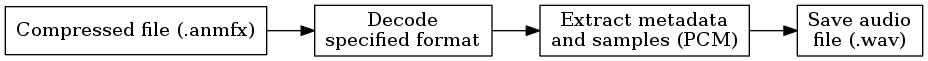
\includegraphics[width=\textwidth]{design_decoder.png}
\end{figure}
